\documentclass{beamer}
\usepackage[T1]{fontenc}
\usepackage[english]{babel}
\usefonttheme{serif}
\setbeamertemplate{navigation symbols}{
\usebeamerfont{footline}
\usebeamercolor[fg]{footline}
\insertframenumber/\inserttotalframenumber{}
}
\setbeamerfont{frametitle}{size = \small}
\usepackage{float}
\usepackage[labelsep = colon]{caption}
\usepackage{amsmath}
\usepackage{setspace}
\usepackage{graphicx}
\usepackage{threeparttablex}
\usepackage{longtable}
\usepackage{booktabs}
\usepackage{dcolumn}
\usepackage{pdfpages}
\usepackage{ulem}
\usepackage{emoji}
\usepackage{fontspec}
\setmainfont{Georgia}

\title{GV217 Conflict, Week 25}
\subtitle{Peacekeeping}
\author{Muzhou Zhang\\ muzhou.zhang@essex.ac.uk\\ Virtual Office Hour: 15:30--16:30, Friday, 997 5800 8679}
\date{25 Mar 2022}

\begin{document}
\maketitle
\setstretch{1.25}

\begin{frame}{Basic Information}
    \begin{itemize}
        \pause\item Number of UNPKOs since 1948?\\
        \pause      71
        \pause\item Number of current UNPKOs?\\
        \pause      12
        \pause\item Number of serving peacekeepers?\\
        \pause      ca. 88,000
        \pause\item Number of fatalities since 1948?\\
        \pause      1,500
        \pause\item Budgets for this fiscal year?\\
        \pause      ca. \$6.3 billion
    \end{itemize}
\end{frame}

\begin{frame}{Basic Information}
    \pause
    \begin{center}
        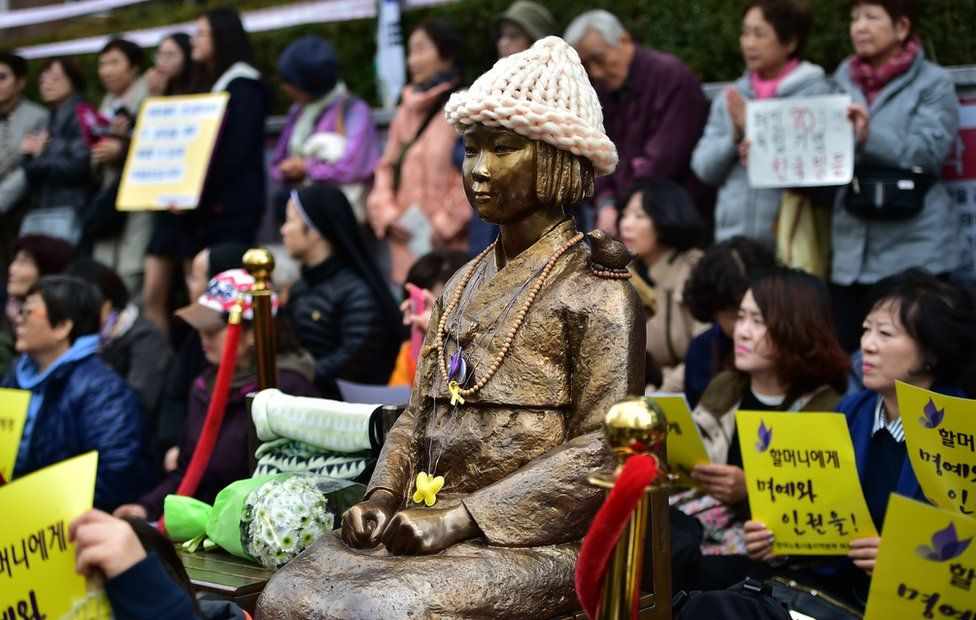
\includegraphics[width = \linewidth]{/Users/mz/Desktop/GitHub/teaching/gv217_conflict_analysis/figs/wk25/fig1.png}
    \end{center}
\end{frame}

\begin{frame}{Basic Information}
    \pause
    \begin{center}
        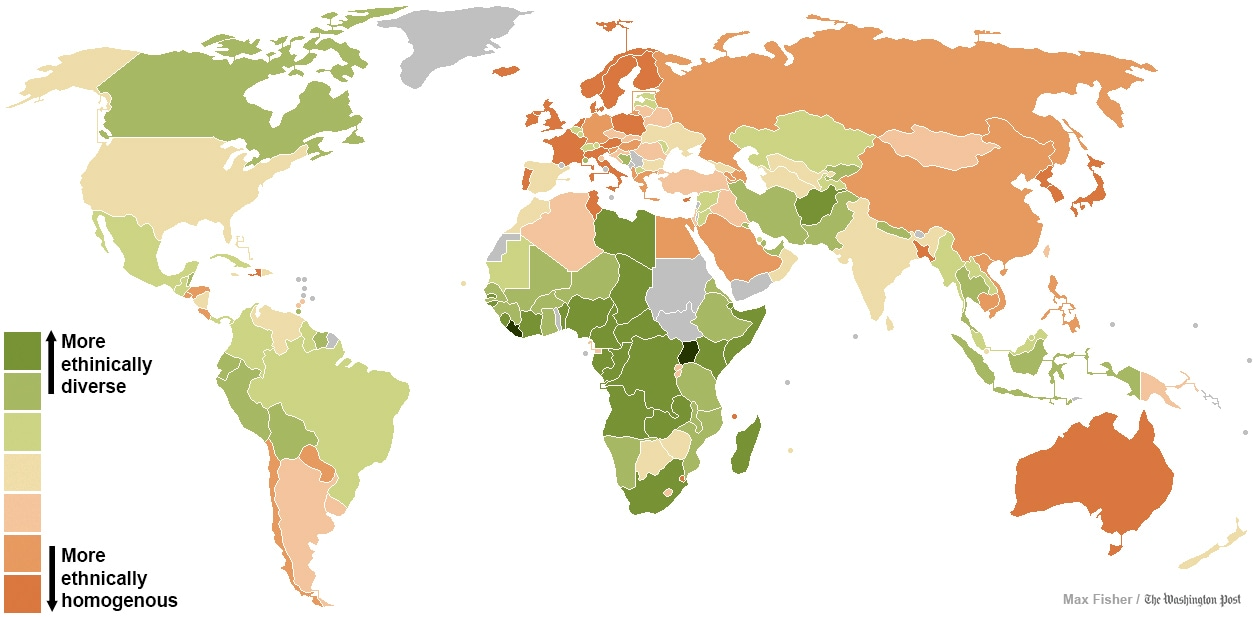
\includegraphics[width = \linewidth]{/Users/mz/Desktop/GitHub/teaching/gv217_conflict_analysis/figs/wk25/fig2.png}
    \end{center}
\end{frame}

\begin{frame}{Basic Information}
    \pause
    \begin{center}
        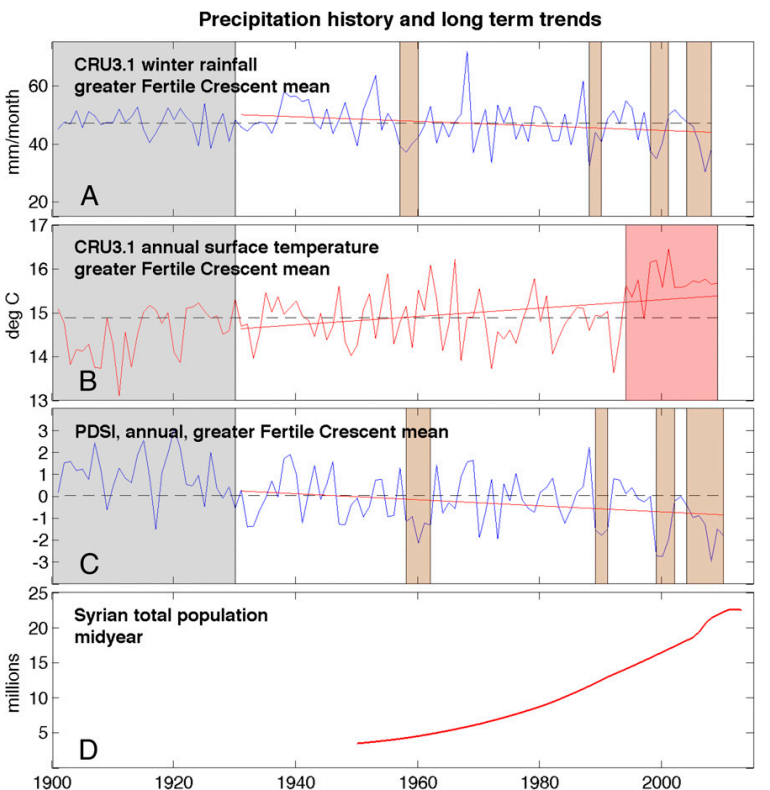
\includegraphics[width = \linewidth]{/Users/mz/Desktop/GitHub/teaching/gv217_conflict_analysis/figs/wk25/fig3.png}
    \end{center}
\end{frame}

\begin{frame}{Key Facts}
\framesubtitle{There are non-UN PKOs}
    \pause
    \begin{center}
        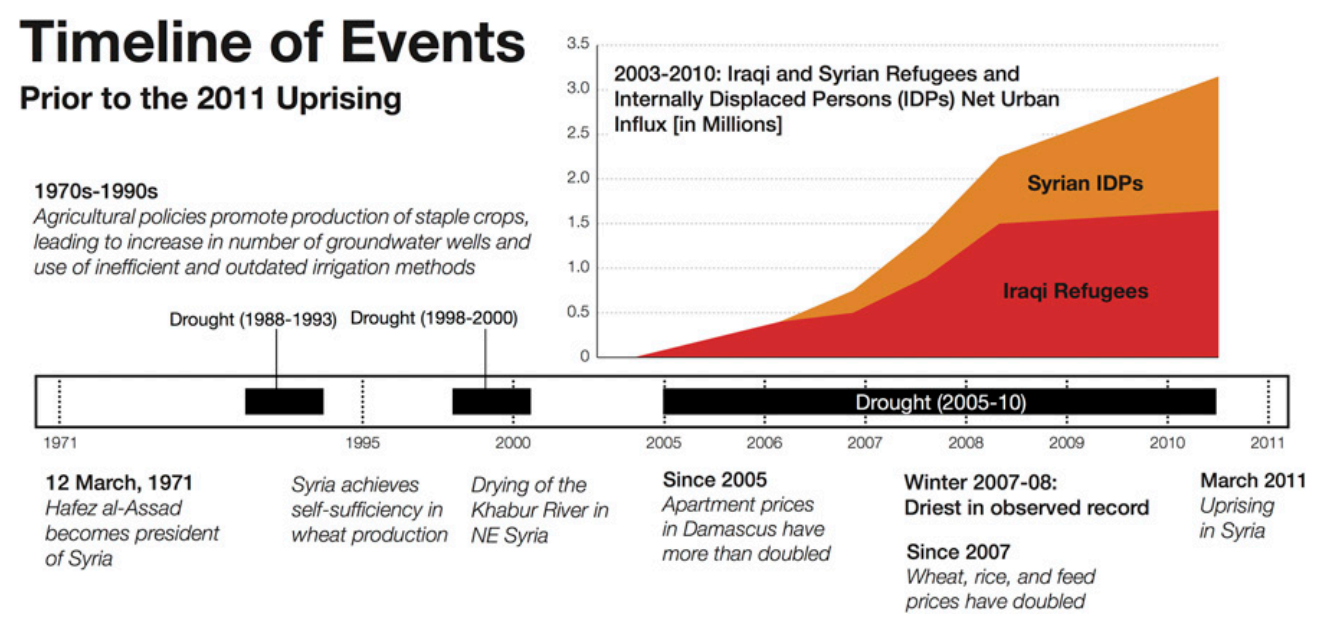
\includegraphics[width = \linewidth]{/Users/mz/Desktop/GitHub/teaching/gv217_conflict_analysis/figs/wk25/fig4.png}
    \end{center}
\end{frame}

\begin{frame}{Key Facts}
\framesubtitle{There are non-military personnel}
    \pause
    \begin{center}
        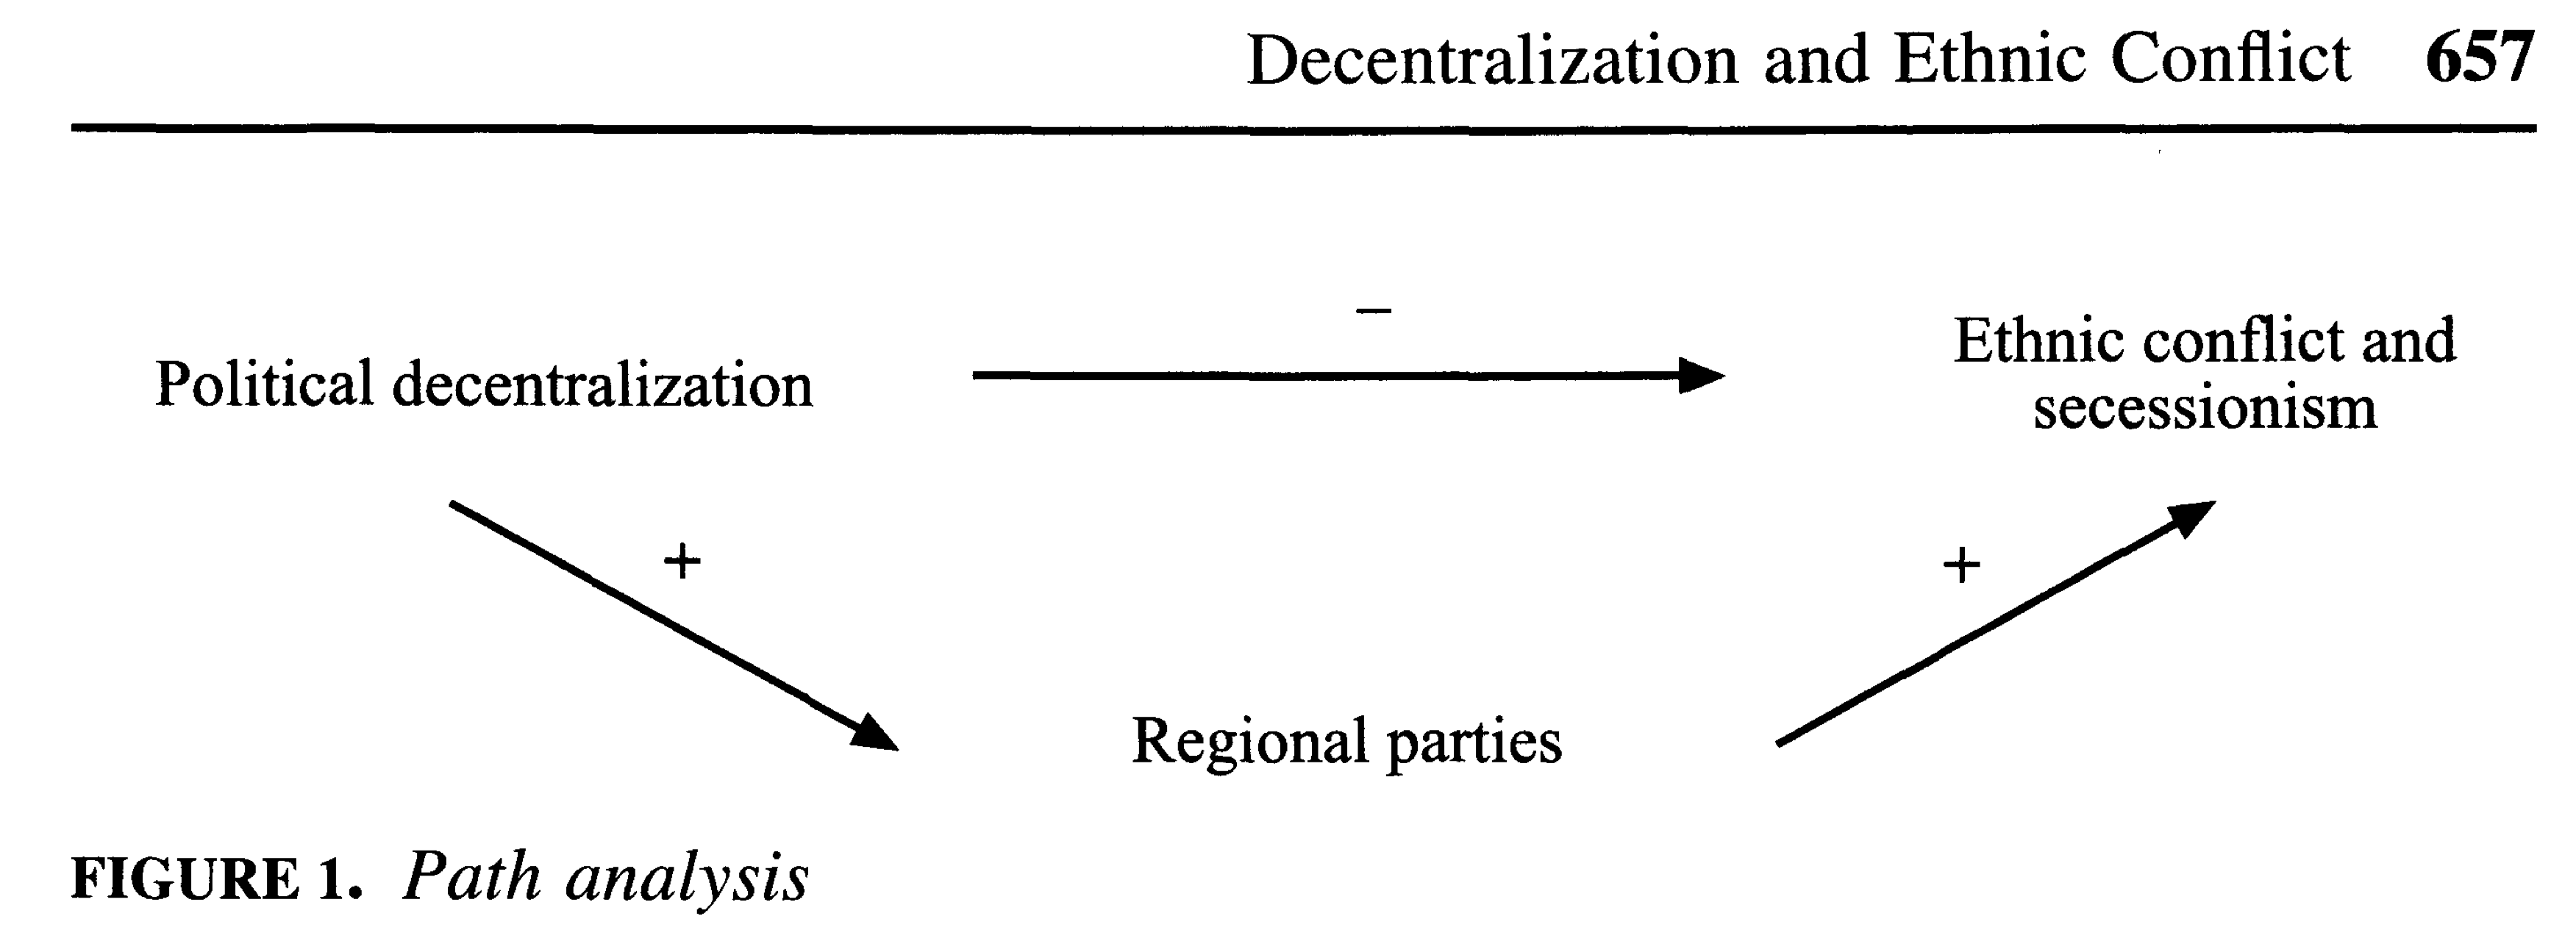
\includegraphics[width = \linewidth]{/Users/mz/Desktop/GitHub/teaching/gv217_conflict_analysis/figs/wk25/fig5.png}
    \end{center}
\end{frame}

\begin{frame}{Key Facts}
    \framesubtitle{UNPKOs are multidimensional}
    \pause
    \begin{center}
        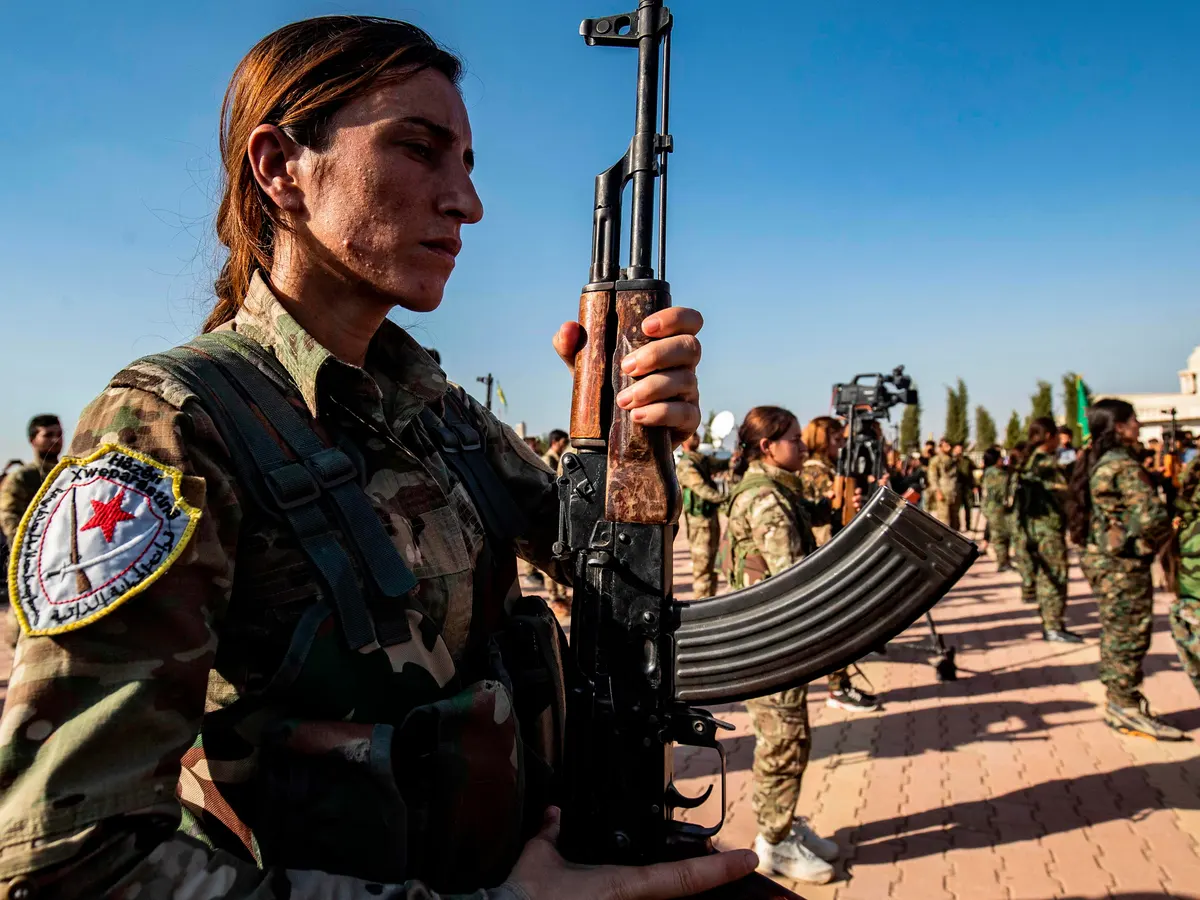
\includegraphics[width = 0.80\linewidth]{/Users/mz/Desktop/GitHub/teaching/gv217_conflict_analysis/figs/wk25/fig6.png}
    \end{center}
    \tiny Di Salvatore (2017, \textit{PhD thesis UvA})
\end{frame}    

\begin{frame}{Supply Side}
\framesubtitle{Top 10 budgets contributors}
\begin{itemize}
    \pause\item \emoji{flag-united-states} United States (27.89\%)
    \pause\item \emoji{flag-china} China (15.21\%)
    \pause\item \emoji{flag-japan} Japan (8.56\%)
    \pause\item \emoji{flag-germany} Germany (6.09\%)
    \pause\item \emoji{flag-united-kingdom} United Kingdom (5.79\%)
    \pause\item \emoji{flag-france} France (5.61\%)
    \pause\item \emoji{flag-italy} Italy (3.30\%)
    \pause\item \emoji{flag-russia} Russian Federation (3.04\%)
    \pause\item \emoji{flag-canada} Canada (2.73\%)
    \pause\item \emoji{flag-south-korea} Republic of Korea (2.26\%)
\end{itemize}
\tiny Fiscal year 2020--2021 (A/C.5/74/18)
\end{frame}

\begin{frame}{Supply Side}
\framesubtitle{Top 10 budgets contributors}
\begin{itemize}
    \pause\item \emoji{flag-bangladesh} Bangladesh (6,403)
    \pause\item \emoji{flag-nepal} Nepal (5,657)
    \pause\item \emoji{flag-india} India (5,598)
    \pause\item \emoji{flag-rwanda} Rwanda (5,280)
    \pause\item \emoji{flag-ethiopia} Ethiopia (4,757)
    \pause\item \emoji{flag-pakistan} Pakistan (3,810)
    \pause\item \emoji{flag-egypt} Egypt (2,795)
    \pause\item \emoji{flag-indonesia} Indonesia (2,697)
    \pause\item \emoji{flag-ghana} Ghana (2,278)
    \pause\item \emoji{flag-china} China (2,243)
\end{itemize}
\tiny As of Jan 31, 2021, \url{https://peacekeeping.un.org/sites/default/files/02_country_ranking_46_jan_2022.pdf}
\end{frame}

\begin{frame}{Supply Side}
\framesubtitle{Some research questions}
\begin{itemize}
    \pause\item Are there free riders?\\
    \pause      Gaibulloev et al. (2015, \textit{JPR}), Passmore, Shannon, \& Hart (2018, \textit{JPR}), Shimuzu \& Sandler (2002, \textit{JPR})
    \pause\item Why countries make PK contributions?\\
    \pause      security concern: Uzonyi (2015, \textit{JPR})\\
    \pause      economic consideration: Zhang (2022, \textit{International Peacekeeping})\\
    \pause      feasibility: Bove \& Elia (2011, \textit{JPR})
\end{itemize}
\end{frame}

\begin{frame}{Evaluating Peacekeeping}
\framesubtitle{Implications}
\begin{itemize}
    \pause\item Security (effectiveness)\\
    \pause      conflict\\
    \pause      violence
    \pause\item Political \& institutional
    \pause\item Economic \& well-being
    \pause\item Environmental
\end{itemize}  
\end{frame}

\begin{frame}{Evaluating Peacekeeping}
\framesubtitle{Empirical Strategy}
\pause
\begin{center}
    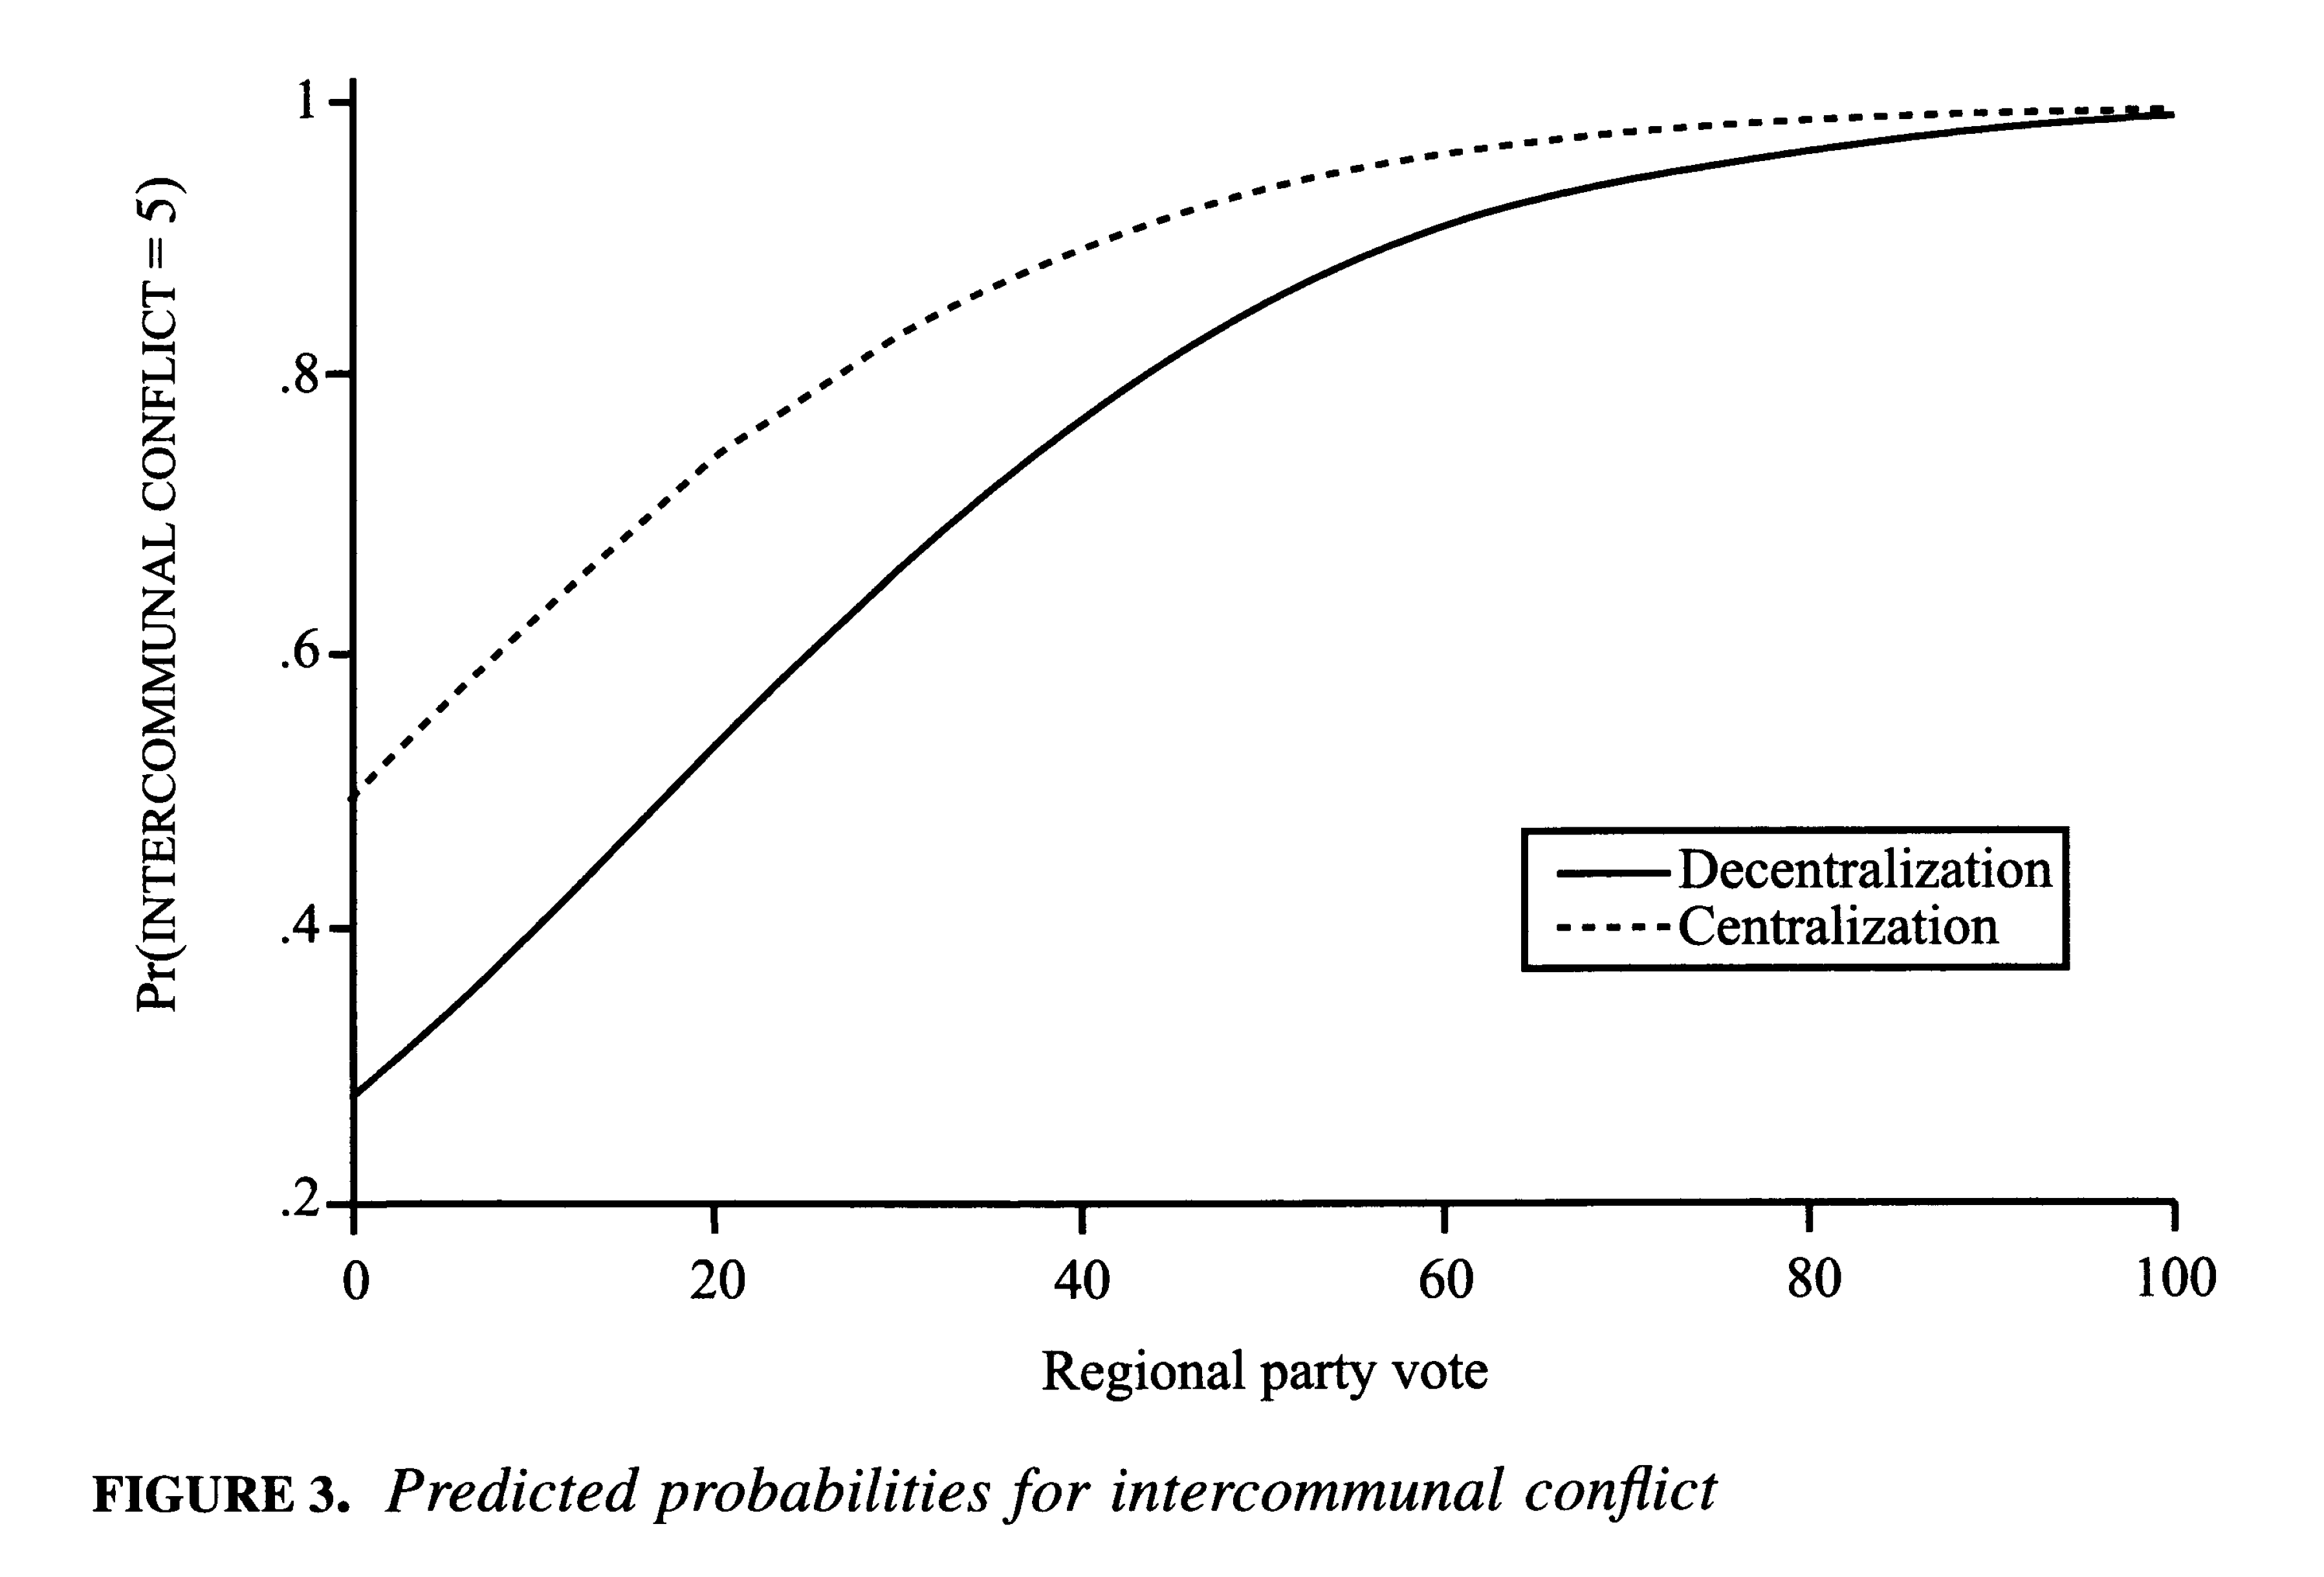
\includegraphics[width = 0.75\linewidth]{/Users/mz/Desktop/GitHub/teaching/gv217_conflict_analysis/figs/wk25/fig7.png}
\end{center}
\tiny Geo-PKO: Cil et al. (2020, \textit{JPR})
\end{frame}

\begin{frame}{Evaluating Peacekeeping}
\framesubtitle{Empirical Strategy}
\pause
\begin{center}
    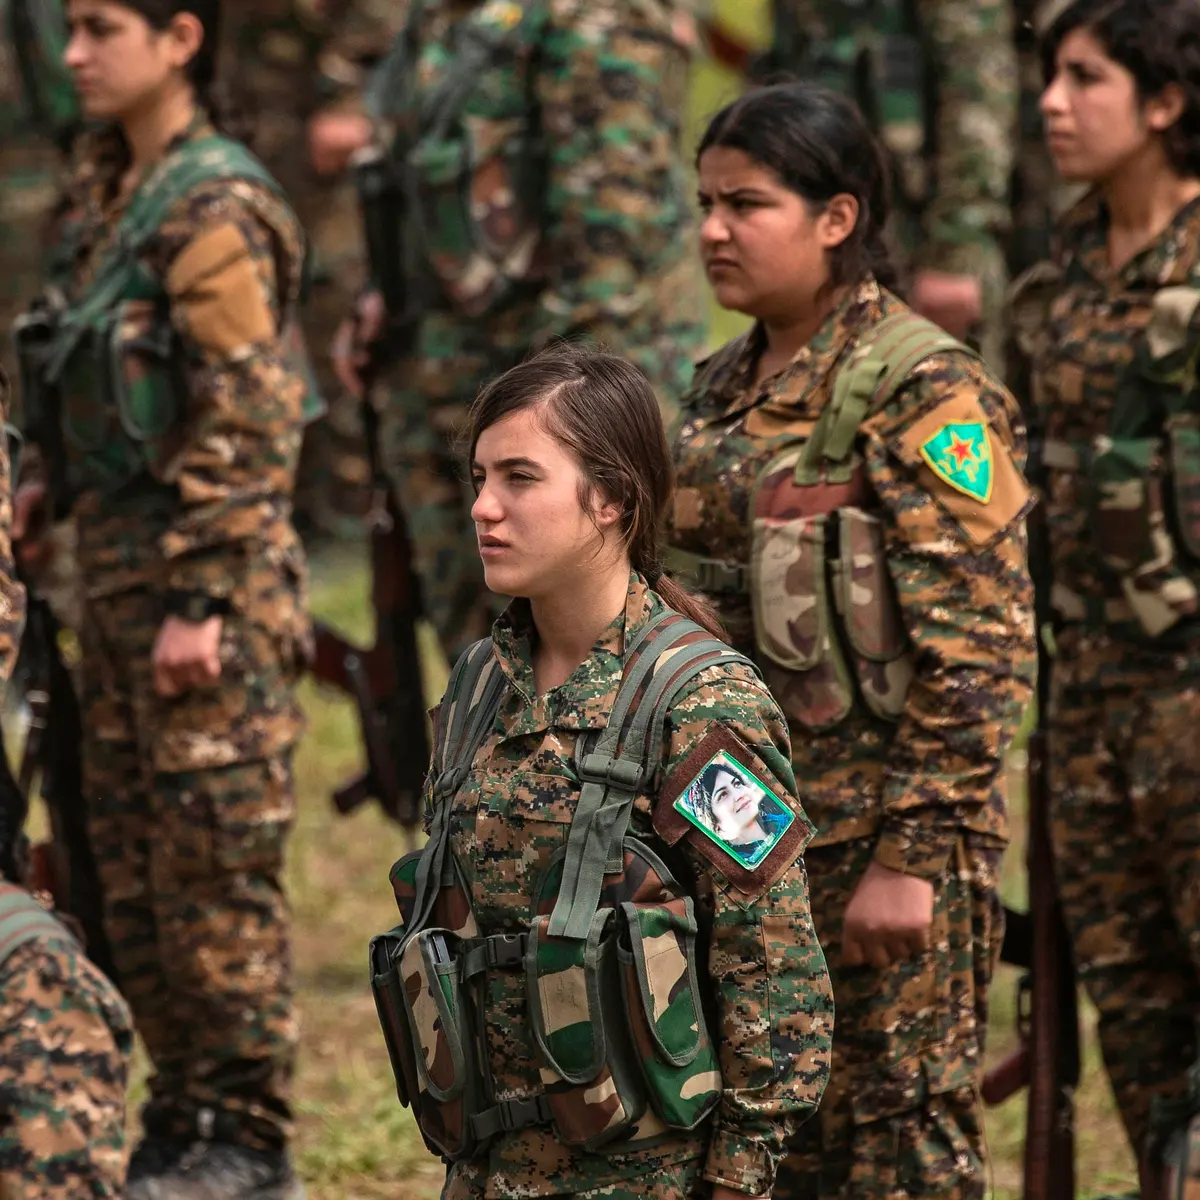
\includegraphics[width = \linewidth]{/Users/mz/Desktop/GitHub/teaching/gv217_conflict_analysis/figs/wk25/fig8.png}
\end{center}
\end{frame}

\begin{frame}{Evaluating Peacekeeping}
\framesubtitle{Empirical Strategy}
\pause PRIO-GRID
\pause
\begin{center}
    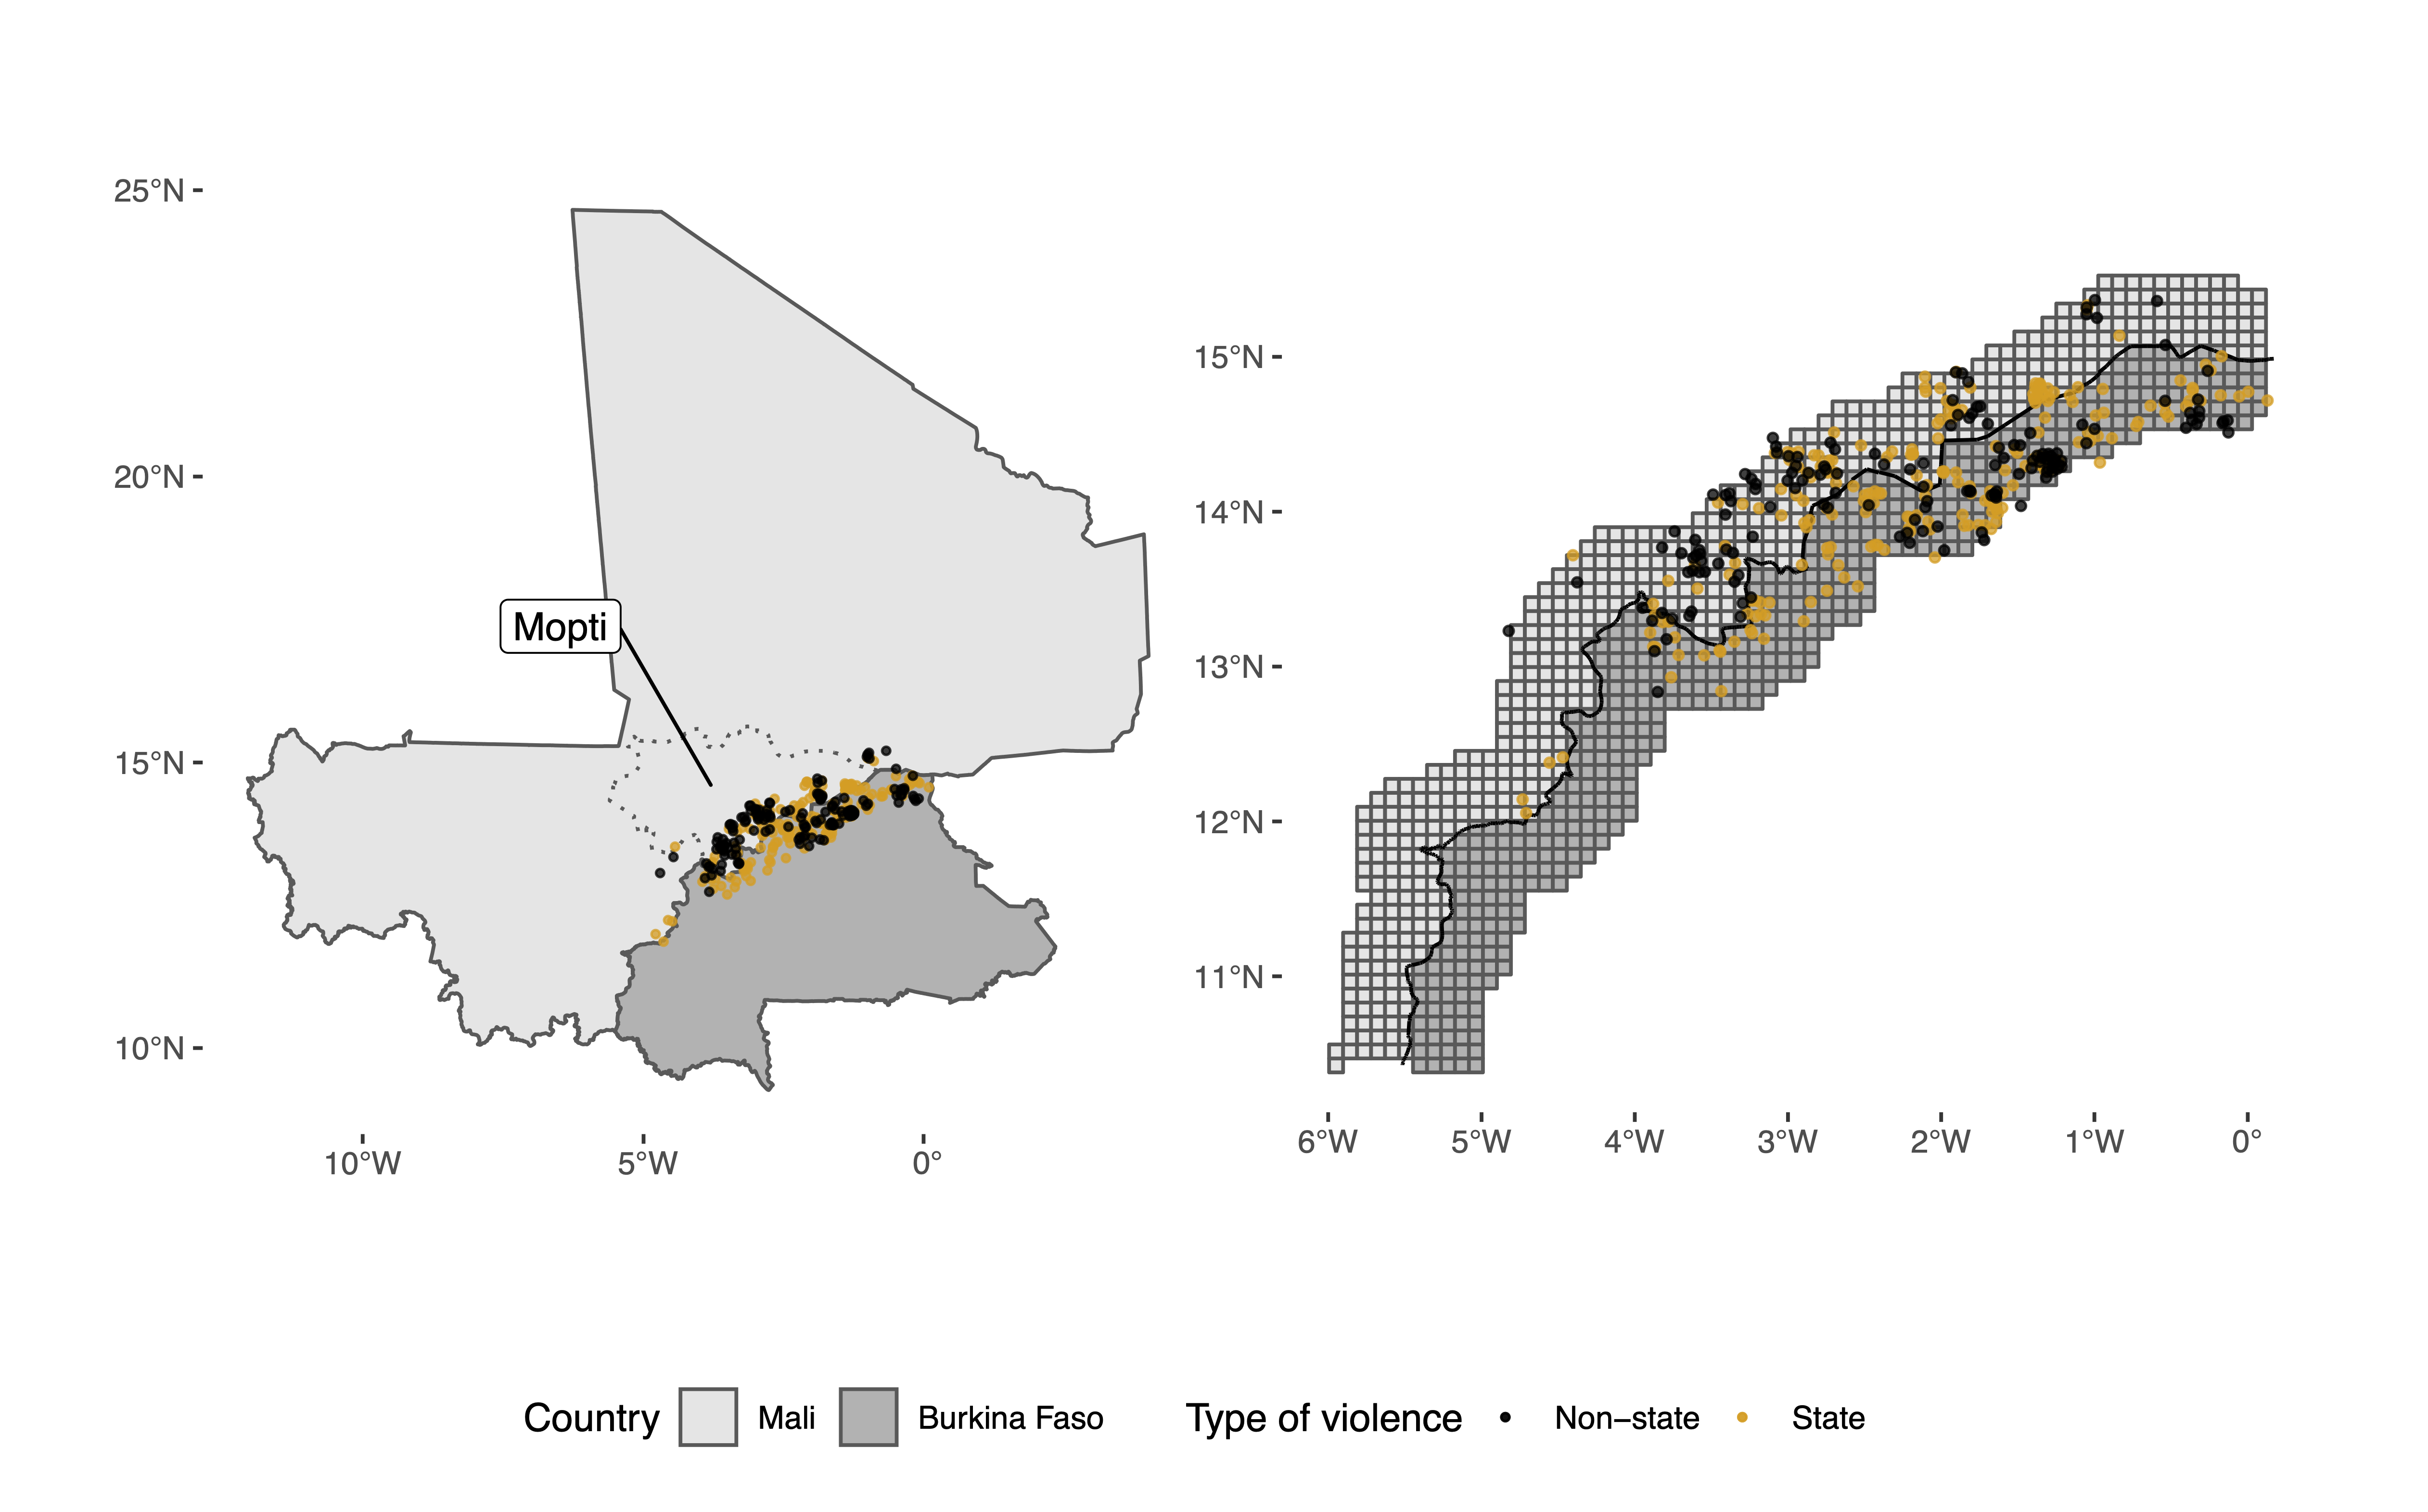
\includegraphics[width = \linewidth]{/Users/mz/Desktop/GitHub/teaching/gv217_conflict_analysis/figs/wk25/fig9.png}
\end{center}
\tiny Nomikos, Şener, \& Williams (2021, \textit{Working Paper})
\end{frame}    

\begin{frame}{Evaluating Peacekeeping}
\framesubtitle{Empirical Strategy}
    \pause Why is causally evaluating PK's implications difficult?\\
    \pause Endogeneity: selection bias
\end{frame}

\begin{frame}{Evaluating Peacekeeping}
\framesubtitle{Making PK more successful}
    \pause How can we know how?\\
    \pause Compare different PKOs with different characteristics
\end{frame}

\end{document}